\section{The automatic bridge}\label{sec:framework}
\ivano{descrizione completa del bridge senza dettagli}
\marco{non so se � sufficiente, gi� sono tre pagine se ci aggiungo pure altre immagini raddoppiamo...}


The concept of bridge is used to denote the capability of interoperability between the UML approach and the DSML one. When a bridge is available for a metamodel and a corresponding profile, it is possible to produce automatically an UML profiled model from a model conforming to the metamodel in question and conversely. In our project we implement a bridge between the metamodels, either between models. The resulting artifacts of the bridge are: a metamodel which represents the profile we are about to translate,  automatically generated transformations which bridge a UML model conforming the profile in question and a model conforming to the brand new generated metamodel.
\begin{figure}[htbp]
	\centering
		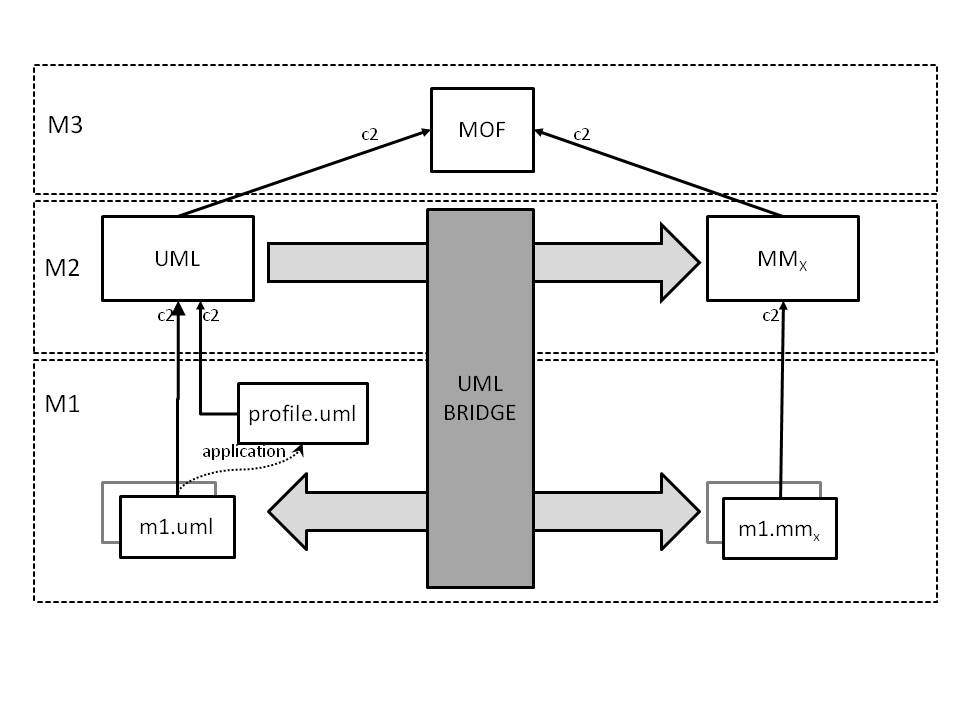
\includegraphics[width=0.80\textwidth]{figures/Diapositiva1.JPG}
	\caption{An overall view of the bridge}
	\label{fig:Diapositiva1}
\end{figure}
In the figure \ref{fig:Diapositiva1},  we have a profile and some profiled models, representing the input artifacts to be transformed, target models are in the right side of the figure, to denote that they are automatically generated. As it can be noticed, the bridging procedure is split in two phases: the first one, works at the metamodeling level by generating a metamodel which is the representation of the profile (and the UML metamodel); the second phase, donw in the figure, works at the modeling level by automatically generating transformations from a profiled UML model to a model which is conform to the brand new generated metamodel.

The resulting metamodel can be considered a union of the UML metamodel (copied in the target one by means of an ad-hoc trasformation superomposed to our one) and the metamodel described in the profile model. We propose a further optimization to our tool which lets the developper to reduce the size of the UML metamodel imported in the target one.

In the following we will show the bridge behaviour at the metamodeling level and at the modeling one. In the end we will show the procedure we propose to slice the obtained metamodel.

\subsection{The bridge at the metamodeling level}\label{sec:metamodelLevel}

At the metamodeling level the bridge takes as input the UML metamodel and the profile. As shown in the figure \ref{fig:Diapositiva1}, it generates a metamodel by coping the UML metamodel in ECORE formalism, and by adding futher constructs which represent the elements in the profile.  The figure \ref{fig:Diapositiva1} represents a UML profile translated into an EMF metamodel. All the UML metamodel elements are in the target metamodel, all the profiled elements (stereotypes and further data types) are represented. The extension mechanism of a stereotype and its metaclass is represented by means of a binding mechanism. Every super class has a reference to the eventual stereotype.
\begin{figure}[htbp]
	\centering
		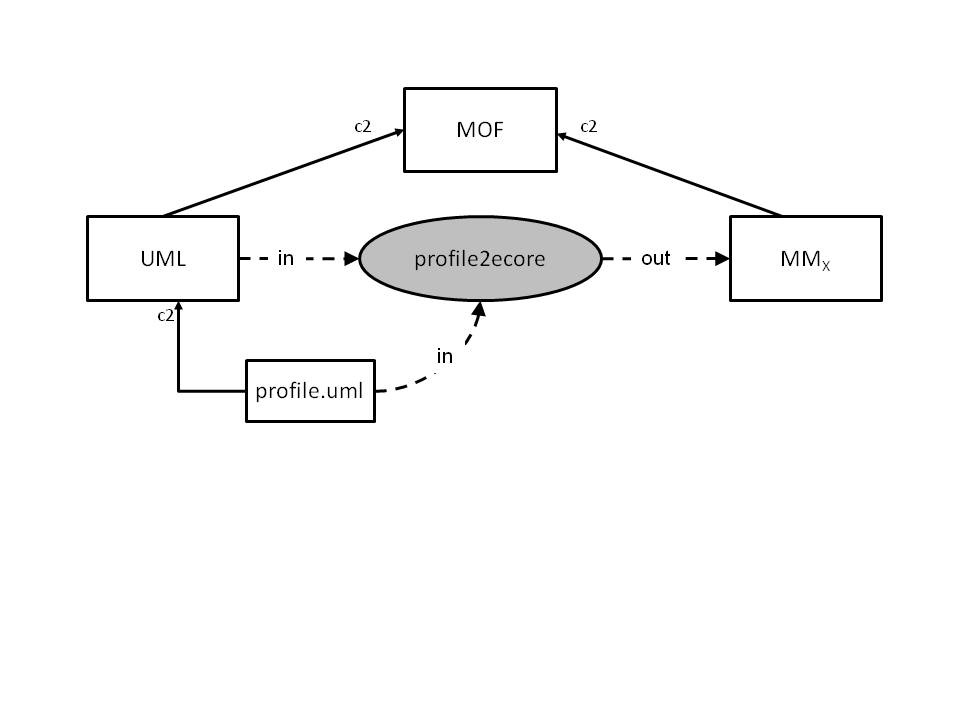
\includegraphics[width=0.80\textwidth]{figures/Diapositiva2.JPG}
	\caption{The bridge at the metamodeling level}
	\label{fig:Diapositiva2}
\end{figure}
In the figure \ref{fig:Diapositiva2} we show the behaviour of our approach. By means of a superimposed transformation we copy the UML metamodel, and we enrich it by adding extension attributes to every metaclasses which has been extended in the profile. The bridge, instead, creates a brand new element bounded with a composition relationship with the metaclasses it extends.

\subsection{The bridge at the modeling level}\label{sec:modeLevel}

At the modeling level the bridge automatically generates transformations which bridge a profiled model in a model conforming to the brand new generated metamodel.
\begin{figure}[htbp]
	\centering
		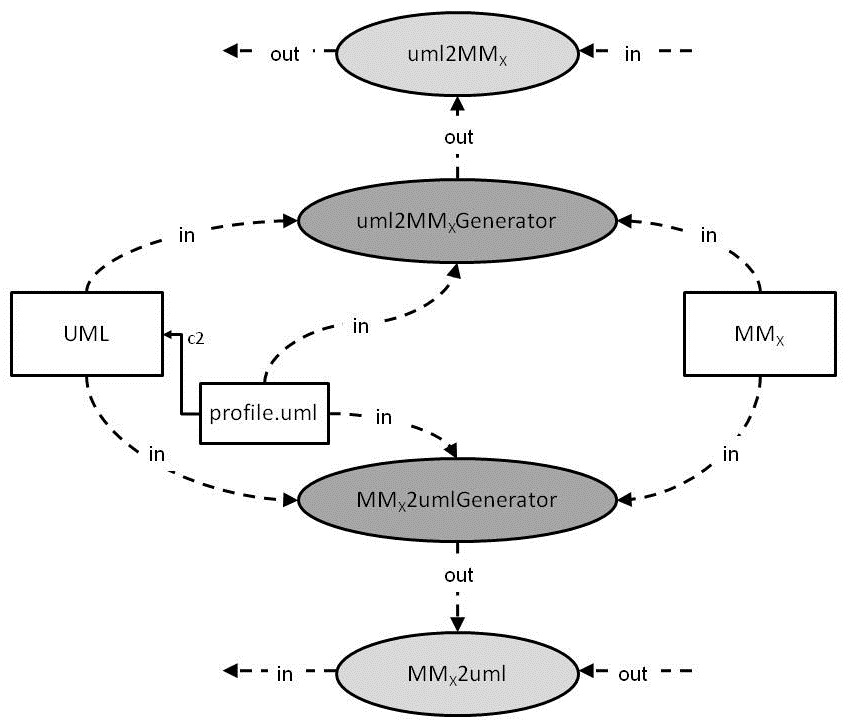
\includegraphics[width=1.00\textwidth]{figures/Diapositiva3.JPG}
	\caption{The bridge at the modeling level}
	\label{fig:Diapositiva3}
\end{figure}
As shown in figure \ref{fig:Diapositiva3}, we used higher order transformations to automatically generate tranformations at the modeling level. The HOT generates a transformations in three phases: (i) in the first one we generate rules to transofrm UML metaclasses into EMF ones; (ii)in the second phase we generate new rules to transform stereotype�s applications into metaclasses�instances representing the stereotype in the target metamodel; (iii) in the last phase we generate imperative code, inserted at the end of every rules generated in the fist phase, to trigger the rules obtained in the second phase. The result is a transformation able to bridge a profiled model in a model conforming to the corresponding brand new genarated metamodel.

By executing this brand new transformation we complete the bridge from UML profiling to EMF metamodeling. 

\section{Slicing the obtained metamodel}\label{sec:slicing}

As previously said, the default behavior of the bridge is to consider the whole UML metamodel and to keep its concepts also in the
target MOF metamodel. On one side this behavior ensures that our bridge is loss-less with respect to the information
provided in the models (it is our primary goal while designing the bridge);
however, on the other side it moves the complexity of the UML metamodel (it contains 246 classes and 583 properties)
into the target MOF metamodel. 
In order to avoid this situation, we couple the bridge with a generic \textbf{slicing algorithm} that allows it to consider  
only the \textit{subset of relevant UML concepts} when passing to the target MOF metamodel.

The subset of relevant UML concepts can be considered as the set of UML metaclasses that can be instantiated in the context of a specific project;
metaclasses outside the relevant set are never instantiated in any model.
A typical example is when designers assume that in the context of a specific project only UML
use case diagrams will be produced; the subset of relevant UML concepts contains only metaclasses 
the can be used in sequence diagrams (e.g., actor, use case, association) and there is no need to keep modeling concepts
for state machines, sequence diagrams, and so on.
This kind of assumptions is recurrent in practice, thus we designed our approach so that the target MOF metamodel contains only 
metaclasses corresponding to relevant UML concepts.
%indeed many UML modeling tools allow to restrict the kind of diagrams that can be created by designers. 

The set of relevant metaclasses is an information related to the target MOF metamodel but it is not included in it (it depends on specific needs of designers). 
Since the slicing algorithm is realized as a model transformation and considering that we were in a MDE context, the set of relevant
metaclasses is represented as an \textit{annotation model}
\footnote{An annotation model is a model containing auxiliary information about another model (the annotated model)\cite{MCDFthesis}} linked to the target MOF metamodel. The annotation model contains a link to each relevant metaclass coming from UML, the slicing algorithm uses those links to identify the metaclasses that will not be sliced out by the slicing procedure.

The current prototype of our approach provides three mechanisms to (semi) automatically obtain the annotation model that will drive the slicing procedure:

\begin{enumerate}
	\item the annotation model is automatically generated from a UML profile;
	\item designers specify only the types of UML diagram they will use, and the corresponding annotation model is automatically generated;
	\item designers provide a set of example UML models, and then the annotation model is automatically generated starting from them.
\end{enumerate}

The mechanisms are implemented as model-to-model transformations (see Section \ref{sec:tool} for more details);
each mechanism has a different level of automation and requires different input artifacts.
For example, if designers already know they will use only specific kinds of UML diagram, then option 2 seems to be the most convenient;
or else, if designers already defined some initial model, they may use the option 3.
Of course, if full control over the generated MOF metamodel is needed, designers can define the annotation model manually, that is they can create an annotation link for each metaclasses that can be instantiated in their UML models.

Once an annotation model is available, then the slicing procedure can be performed;
it is based on a generic slicing algorithm for MOF metamodels~\cite{ICSEbyadl}. Let
$MM$ be a metamodel and let $SC$ be a subset of the elements in
$MM$; $slice$ is defined as follows:

\vspace{-.2cm}
$$slice(SC)=SC \cup \displaystyle\bigcup_{c \in
SC}{slice(neighbour(c))}$$
\vspace{-.2cm}

\noindent where $neighbour(c)$ is the set of all superclasses of
$c$, of all classes referred (both with association and
aggregation) by $c$, and of all types of attributes in $c$. 
It is important to note that even though $slice$ is defined
as a set of classes, since each class contains also references
to other classes, the final result is a subset of the metamodel $MM$
with both classes and their relations.
%
\begin{figure}
  \centering
  \subfloat[]{\label{fig:slicerMM}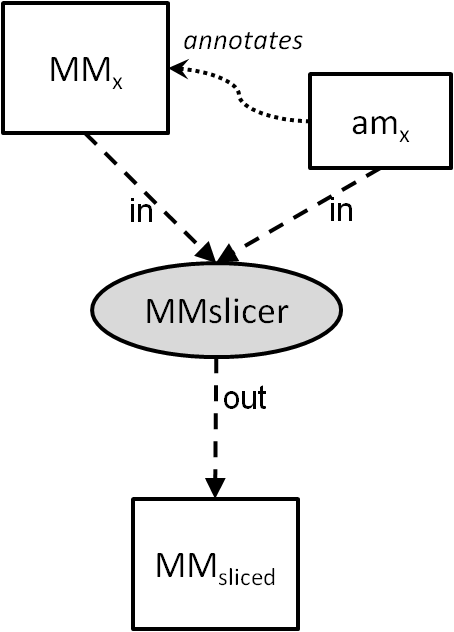
\includegraphics[scale=0.4]{figures/slicerMM}}      
 \hspace{10mm}          
  \subfloat[]{\label{fig:slicerT}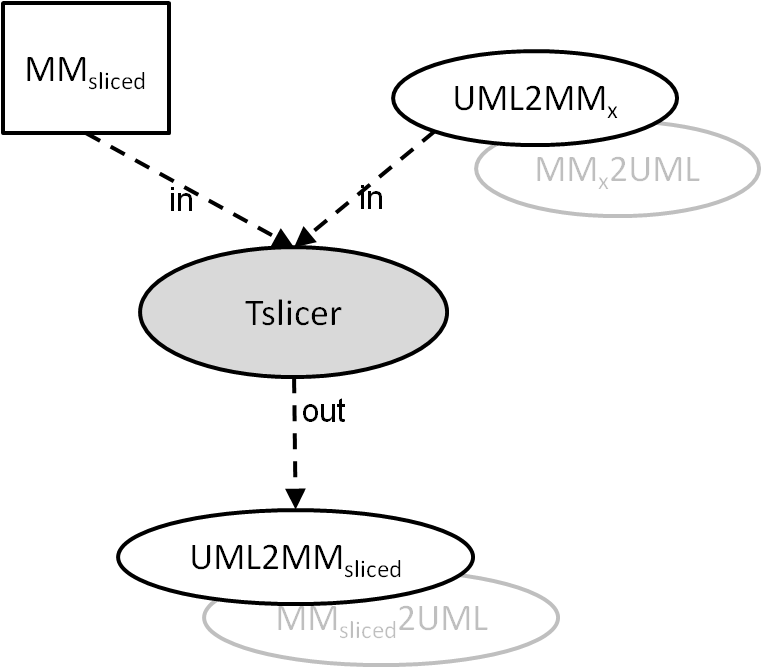
\includegraphics[scale=0.4]{figures/slicerT.png}}
  \caption{Slicing the MOF metamodel (a) and the generated transformations (b)}
  \label{fig:animals}
\end{figure}
%
As can be seen in Figure \ref{fig:slicerMM}, the slicing algorithm is realized as a model-to-model transformation called \textit{MMslicer}.
It that takes as input a MOF metamodel $MM_x$ and an annotation model $am_x$, and generates a new metamodel $MM_sliced$ containing 
a subset of $MM_x$ according to the metaclasses referenced in $am_x$.

At this point we must consider a possible issue that may arise: once the target MOF metamodel has been sliced, the
previously generated model transformations of the bridge may refer to missing metaclasses in the metamodel.
This implies that our approach must provide a mechanism for adapting also the $UML2MM_x$ and $MM_x2UML$ transformations
to the newly sliced metamodel.
We are aware that in literature there are generic approaches managing the coupled evolution of metamodels and model transformations
\cite{CITATION1}\cite{CITATION2}; however, since in our case we can assume that elements 
\begin{center}

\end{center}
can be only deleted from metamodels (we do not need to manage neither additions or updates), and since we need a fully automatic mechanism, we developed our minimalistic solution to automatically adapt model transformations to sliced metamodels.
Our solution takes inspiration from the EMFMigrate project\footnote{EMFMigrate project website: \small{\url{http://www.emfmigrate.org}}}
and it is based on an higher-order transformation; in this work we call it $Tslicer$.
%This kind of issue is well-known in the metamodel co-evolution research field \cite{CITAZIONI}, \footnote{http://www.emfmigrate.org}

Figure \ref{fig:slicerT} gives an idea of how the \textit{Tslicer} transformation works. It takes as input (i) the sliced metamodel
($MM_sliced$ in figure) and (ii) the model transformation to be adapted ($UML2MM_x$ in figure). $Tslicer$ automatically adapts the input transformation according to the meta-elements (i.e., metaclasses, attributes, references) 
that were previously sliced out from $MM_sliced$. The grey elements in Figure \ref{fig:slicerT} show that $Tslicer$ can also be
applied on the transformation in the other direction (i.e., $MM_x2UML$); this ensures that using the slicing algorithm does not affect
the bridge in terms of automation and bidirectionality. More details on $Tslicer$ are provided in Section \ref{sec:tool}.

In conclusion, it is important to note that the whole slicing mechanism (both on metamodels and transformations) 
acts as a post-processing activity of the artifacts generated by the bridge described in Section \ref{sec:framework}; this means that, according to project-specific needs, the proposed bridge and slicing mechanism can be used independently.
%Intuitively, it copies all the elements of the input transformation (like transformation rules, imperative statements, conditions, and so on)
%and ignores those elements that reference a meta-element  that are not in $MM_sliced$ anymore.

%removes those elements of the input model transformation (e.g., transformation rules, imperative statements, conditions)
%that reference a meta-element that is not in $MM_sliced$ anymore (i.e., such an element has been sliced out by $Mslicer$).  

